\section{Parsing of JPEG bytestream}
Initially the data generated from \gs was piped through \code{stdout}.
The following binary \gls{regex} was used in to separate the images.
\begin{figure}[H]
    \centering
    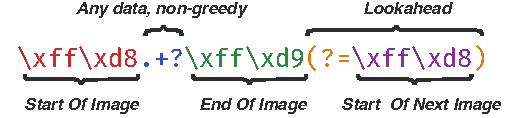
\includegraphics[width=0.7\textwidth]{figures/jpeg_regex.pdf}
\end{figure}
It looked for the beginning marker followed by data followed by the end marker and with a lookahead for the beginning marker of the next image.
The final lookahead was used to minimize the chance of parsing data bytes as the end marker as it was believed that could happen.
After analyzing the \gls{jpeg} standard however it was discovered that they use a technique called byte stuffing which ensures this never happens \cite[91]{ccittINFORMATIONTECHNOLOGYDIGITAL1992}.
Byte stuffing is a technique used in data transmission where special control characters are inserted into the data stream to distinguish between data and control information.
For \glspl{jpeg}, the zero byte is inserted after every control character that appears in the data \cite[91]{ccittINFORMATIONTECHNOLOGYDIGITAL1992}.
This made the parsing could be done both easier and faster by simply reading until the end-of-image marker.